\documentclass[manuscript,screen,nonacm]{acmart}
\usepackage{tikz}
\tikzset{>=latex}
\usetikzlibrary{patterns}
\usepackage{colortbl}
\usetikzlibrary{calc}

\begin{document}

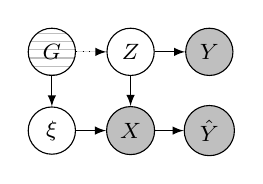
\begin{tikzpicture}
\footnotesize{
\node (g) [circle, draw, fill=gray!50!white, minimum size=0.6cm,pattern=horizontal lines, pattern color=gray!50!white] {$G$};
\node (z) [circle, draw, fill=white, right of=g, minimum size=0.6cm] {$Z$};
\node (y) [circle, draw, fill=gray!50!white, right of=z, minimum size=0.6cm] {$Y$};
\node (xi) [circle, draw, fill=white, below of=g, minimum size=0.6cm] {$\xi$};
\node (x) [circle, draw, fill=gray!50!white, right of=xi, minimum size=0.6cm] {$X$};
\node (haty) [circle, draw, fill=gray!50!white, right of=x, minimum size=0.6cm] {$\hat{Y}$};

\draw[dotted,->,black,fill=black] (g) -- (z);
\draw[->,black,fill=black] (z) -- (y);
\draw[->,black,fill=black] (xi) -- (x);
\draw[->,black,fill=black] (x) -- (haty);
\draw[->,black,fill=black] (g) -- (xi);
\draw[->,black,fill=black] (z) -- (x);
}
\end{tikzpicture}

\end{document}